\documentclass{standalone}
\usepackage{graphicx}	
\usepackage{amssymb, amsmath}
\usepackage{color}

\usepackage{tikz}
\usetikzlibrary{intersections, backgrounds}
\usepackage{pgfmath}

\definecolor{light}{RGB}{220, 188, 188}
\definecolor{mid}{RGB}{185, 124, 124}
\definecolor{dark}{RGB}{143, 39, 39}
\definecolor{highlight}{RGB}{180, 31, 180}
\definecolor{gray10}{gray}{0.1}
\definecolor{gray20}{gray}{0.2}
\definecolor{gray30}{gray}{0.3}
\definecolor{gray40}{gray}{0.4}
\definecolor{gray60}{gray}{0.6}
\definecolor{gray70}{gray}{0.7}
\definecolor{gray80}{gray}{0.8}
\definecolor{gray90}{gray}{0.9}
\definecolor{gray95}{gray}{0.95}

\begin{document}

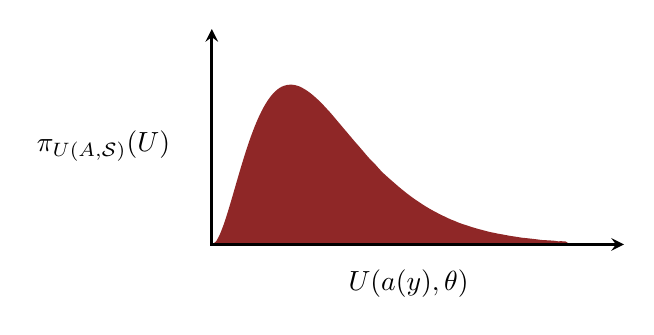
\begin{tikzpicture}[scale=0.5, thick,
declare function={ g(\x) = 0.5 * (\x * \x) * exp(-\x);}
]
  \fill[color=dark, domain=0:10, smooth, samples=100, variable=\x] 
    plot ({\x}, {15 * g(\x)});

  \node[] at (-2.75, 2.5) { $\pi_{U(A, \mathcal{S})} (U)$ };

  \draw [->, >=stealth, line width=1] (-0.03, 0) -- +(10.5, 0);
  \draw [->, >=stealth, line width=1] (-0, -0.03) -- +(0, 5.5);
  \node[] at (5, -1) { $U(a(y), \theta)$ };
  
  
  
\end{tikzpicture}

\end{document}  